\vspace{-0.15in}

\section{Background}
\label{sec:Background}

\vspace{-0.1in}

%\subsection{DREMS Components:}
%\label{sec:drems_component}

%\vspace{-0.05in}
\textbf{DREMS Components:}
Design and implementation of component-based software applications rests on the principle of assembly: \textit{Complex systems are built by composing re-useable interacting components}. Components contain functional, business-logic code that implements operations on state variables. Ports facilitate interactions between communicating components. A component-level message queue, with associated infrastructure code, controls the scheduling of operations of the individual components. Figure \ref{fig:drems_component} shows the basic DREMS component.

Each DREMS component supports four basic types of ports for interaction with other collaborating components: Facets, Receptacles, Publishers and Subscribers. A component's {\bf facet} is a unique interface that can be invoked either synchronously via remote method invocation (RMI) or asynchronously via asynchronous method invocation (AMI). A component's {\bf receptacle} specifies an interface required by the component in order to function correctly. Using its receptacle, a component can invoke operations on other components using either RMI or AMI. A {\bf publisher} port is a single point of data emission and a {\bf subscriber} port is a single point of data consumption. Communication between publishers and subscribers is contingent on the compatibility of their associated topics (i.e. data types). More details on this component model can be found in \cite{ISIS_F6_ISORC:13}.

%\vspace{-0.2in}

\begin{figure}[t]
	\centering
	\begin{subfigure}[b]{0.5\textwidth}
		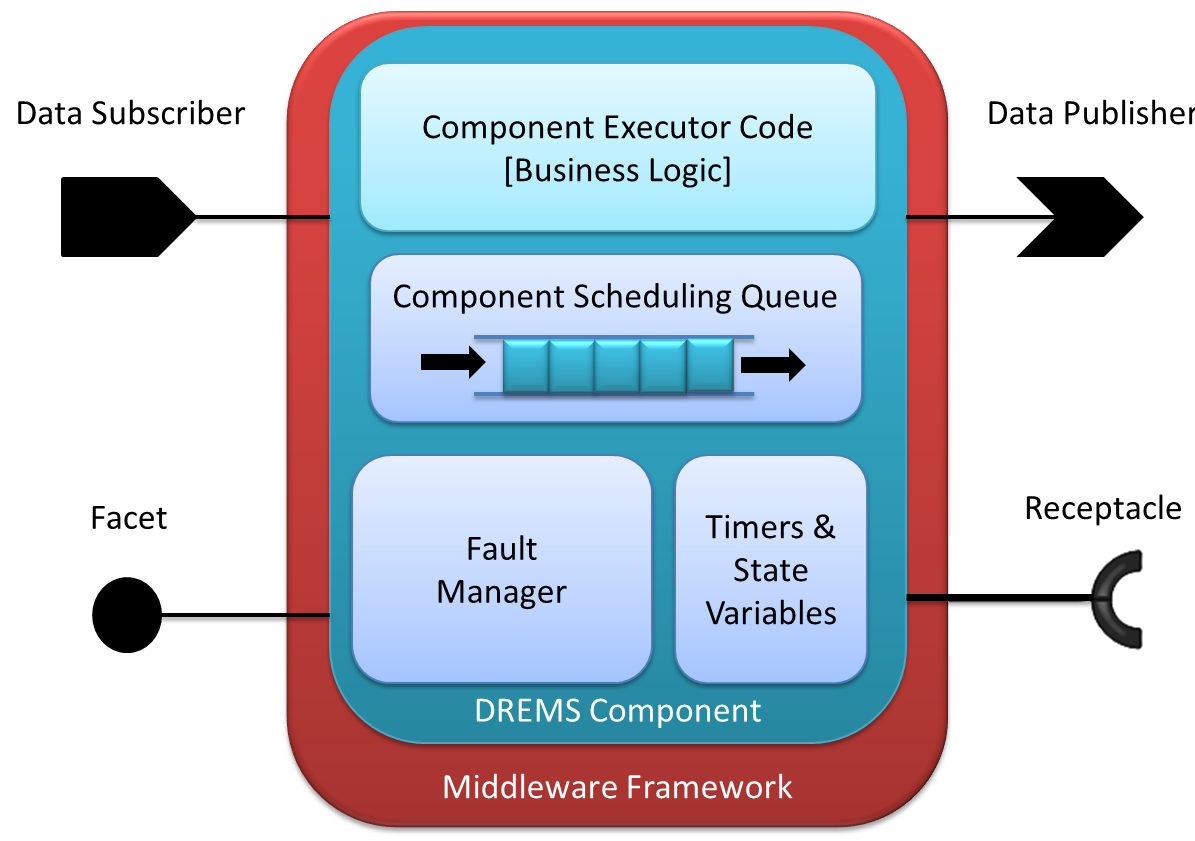
\includegraphics[width=\textwidth]{./figs/drems_component}
		\caption{DREMS Component}
		\label{fig:drems_component}
	\end{subfigure}%
	\begin{subfigure}[b]{0.5\textwidth}
		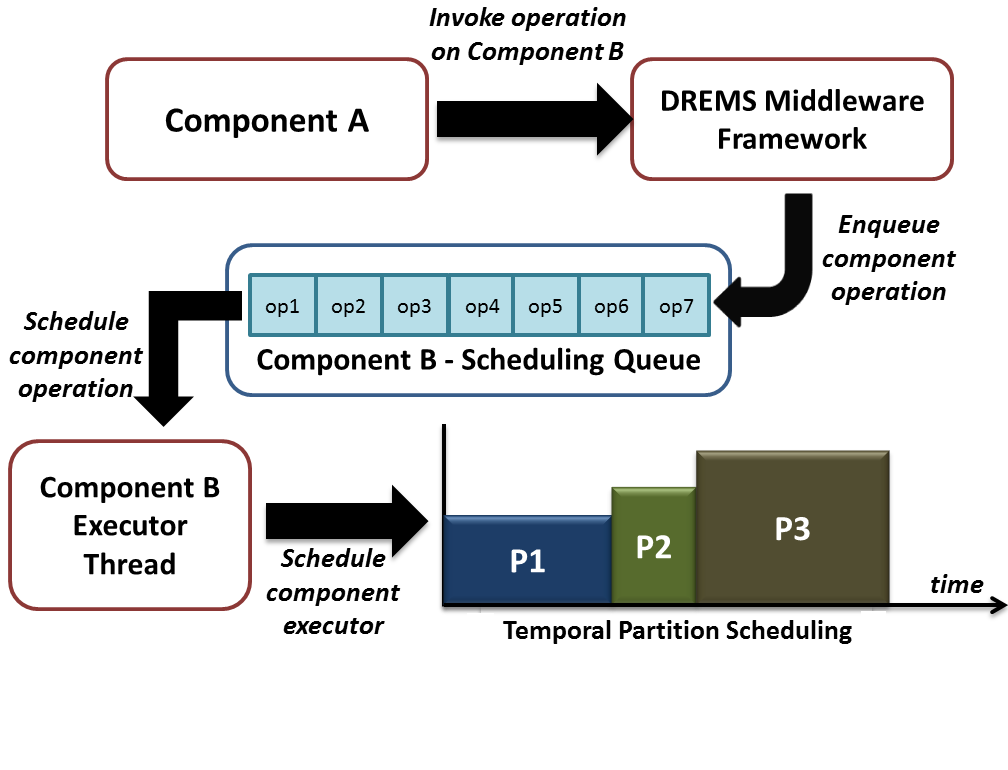
\includegraphics[width=\textwidth]{./figs/component_operations}
		\caption{Component Operation Scheduling}
		\label{fig:component_operations}
	\end{subfigure}
	\caption{DREMS Infrastructure}\label{fig:DI}
\vspace{-0.2in}
\end{figure}


\noindent
\textbf{Component Operation Scheduling:}
%\label{sec:component_operations}
%\vspace{-0.1in}
 An operation is an abstraction for the different tasks undertaken by a component. These tasks are implemented by the component's executor code written by the developer. As shown in Figure \ref{fig:component_operations}, in order to service interactions with the underlying framework and with other components, every component is associated with a message queue. This queue holds instances of operations ('messages') that are ready for execution and need to be serviced by the component. These operations service either interaction requests (seen on communication ports) or service requests (from the underlying framework). An example for the latter is the use of component timers that can periodically (or sporadically) activate an operation. Each operation is characterized by a priority and a deadline. The deadline here is the maximum acceptable time between the release of a component operation and the completion of that operation, measured starting from when the operation is enqueued onto the component's message queue.
To facilitate component behavior that is free of deadlocks and race conditions, the component's execution is handled by a single thread. This single-threaded execution helps avoid synchronization primitives such as internal lock variables that lead to tenuous code development.

The DREMS OS scheduler enforces an ARINC-653 ~\cite{ARINC-653} style temporal and spatial partition scheme in order to schedule components grouped into processes. Temporal partitions, as shown in Figure \ref{fig:component_operations}, are periodic fixed intervals of the processor time. Note that there are two levels of scheduling in DREMS: (1) Each component operation in the component-level is scheduled using a component-level scheduler, and (2) each component executor thread, on the system-level, is scheduled by the OS in one of the temporal partitions, granting a slice of the CPU's time to those threads.

\vspace{-0.2in}

\subsection{Colored Petri Nets}

\vspace{-0.1in}

Petri nets \cite{Murata1989} are a graphical modeling tool used for describing and analyzing a wide range of systems. A Petri net is a five-tuple $(P, T, A, W, M0)$ where P is a finite set of places, T is a finite set of transitions, A is a finite set of arcs between places and transitions, W is a function assigning weights to arcs, and M0 is the initial marking of the net. Places hold a discrete number of markings called tokens.  
A transition can legally fire when all of its input places have necessary number of tokens, and when fires it produces tokens for its output places. 

With Colored Petri nets (CPN) \cite{CPN}, tokens carry values of specific data types called colors. Transitions in CPN are enabled for firing only when valid colored tokens are present in all of the typed input places, and valid arc bindings are realized to produce the necessary colored tokens on the output places. The firing of transitions in CPN can check for and modify the data values of these colored tokens. Furthermore, large and complex models can be constructed by composing smaller sub-models as CPN allows for hierarchical description. This extended paradigm can more easily model and analyze systems with typed parameters. 
